% ==============================================================================
% ACDE SYSTEM ARCHITECTURE SPECIFICATION FOR IEEE TRANSACTIONS JOURNAL
% Derived strictly from the ground-truth codebase (src/acde, infra/, schemas)
% ==============================================================================

\section{System Architecture and Formal Control Specification}
\label{sec:architecture}

The Autonomous Cloud Data Engineering (\textsc{Acde}) framework is structured as a decoupled, policy-bounded supervisory control plane designed to govern mission-critical heterogeneous cloud data pipelines. Conventional data pipeline management oscillates between passive observability stacks (which lack remediation agency) and opaque autonomous agents (which execute arbitrary actions and synthesize unverified code). In contrast, \textsc{Acde} enforces a strict architectural boundary: \emph{agents reason and propose; formal declarative policies decide; deterministic execution engines enforce}. 

Fig.~\ref{fig:system_architecture} illustrates the overarching seven-layer architecture of \textsc{Acde}, highlighting the strict separation between non-deterministic cognitive reasoning and deterministic operational enforcement.

% ------------------------------------------------------------------------------
% FIGURE: COMPLETE SYSTEM ARCHITECTURE (TIKZ / VECTOR SCHEMATIC)
% ------------------------------------------------------------------------------
% OPTION A: INCLUDE VECTOR PDF / HIGH-RES PNG (RECOMMENDED VISIO-STYLE PUBLICATION FIGURE)
% To use the generated Visio-style vector figure directly in your paper, uncomment below:
%
% \begin{figure*}[!t]
% \centering
% 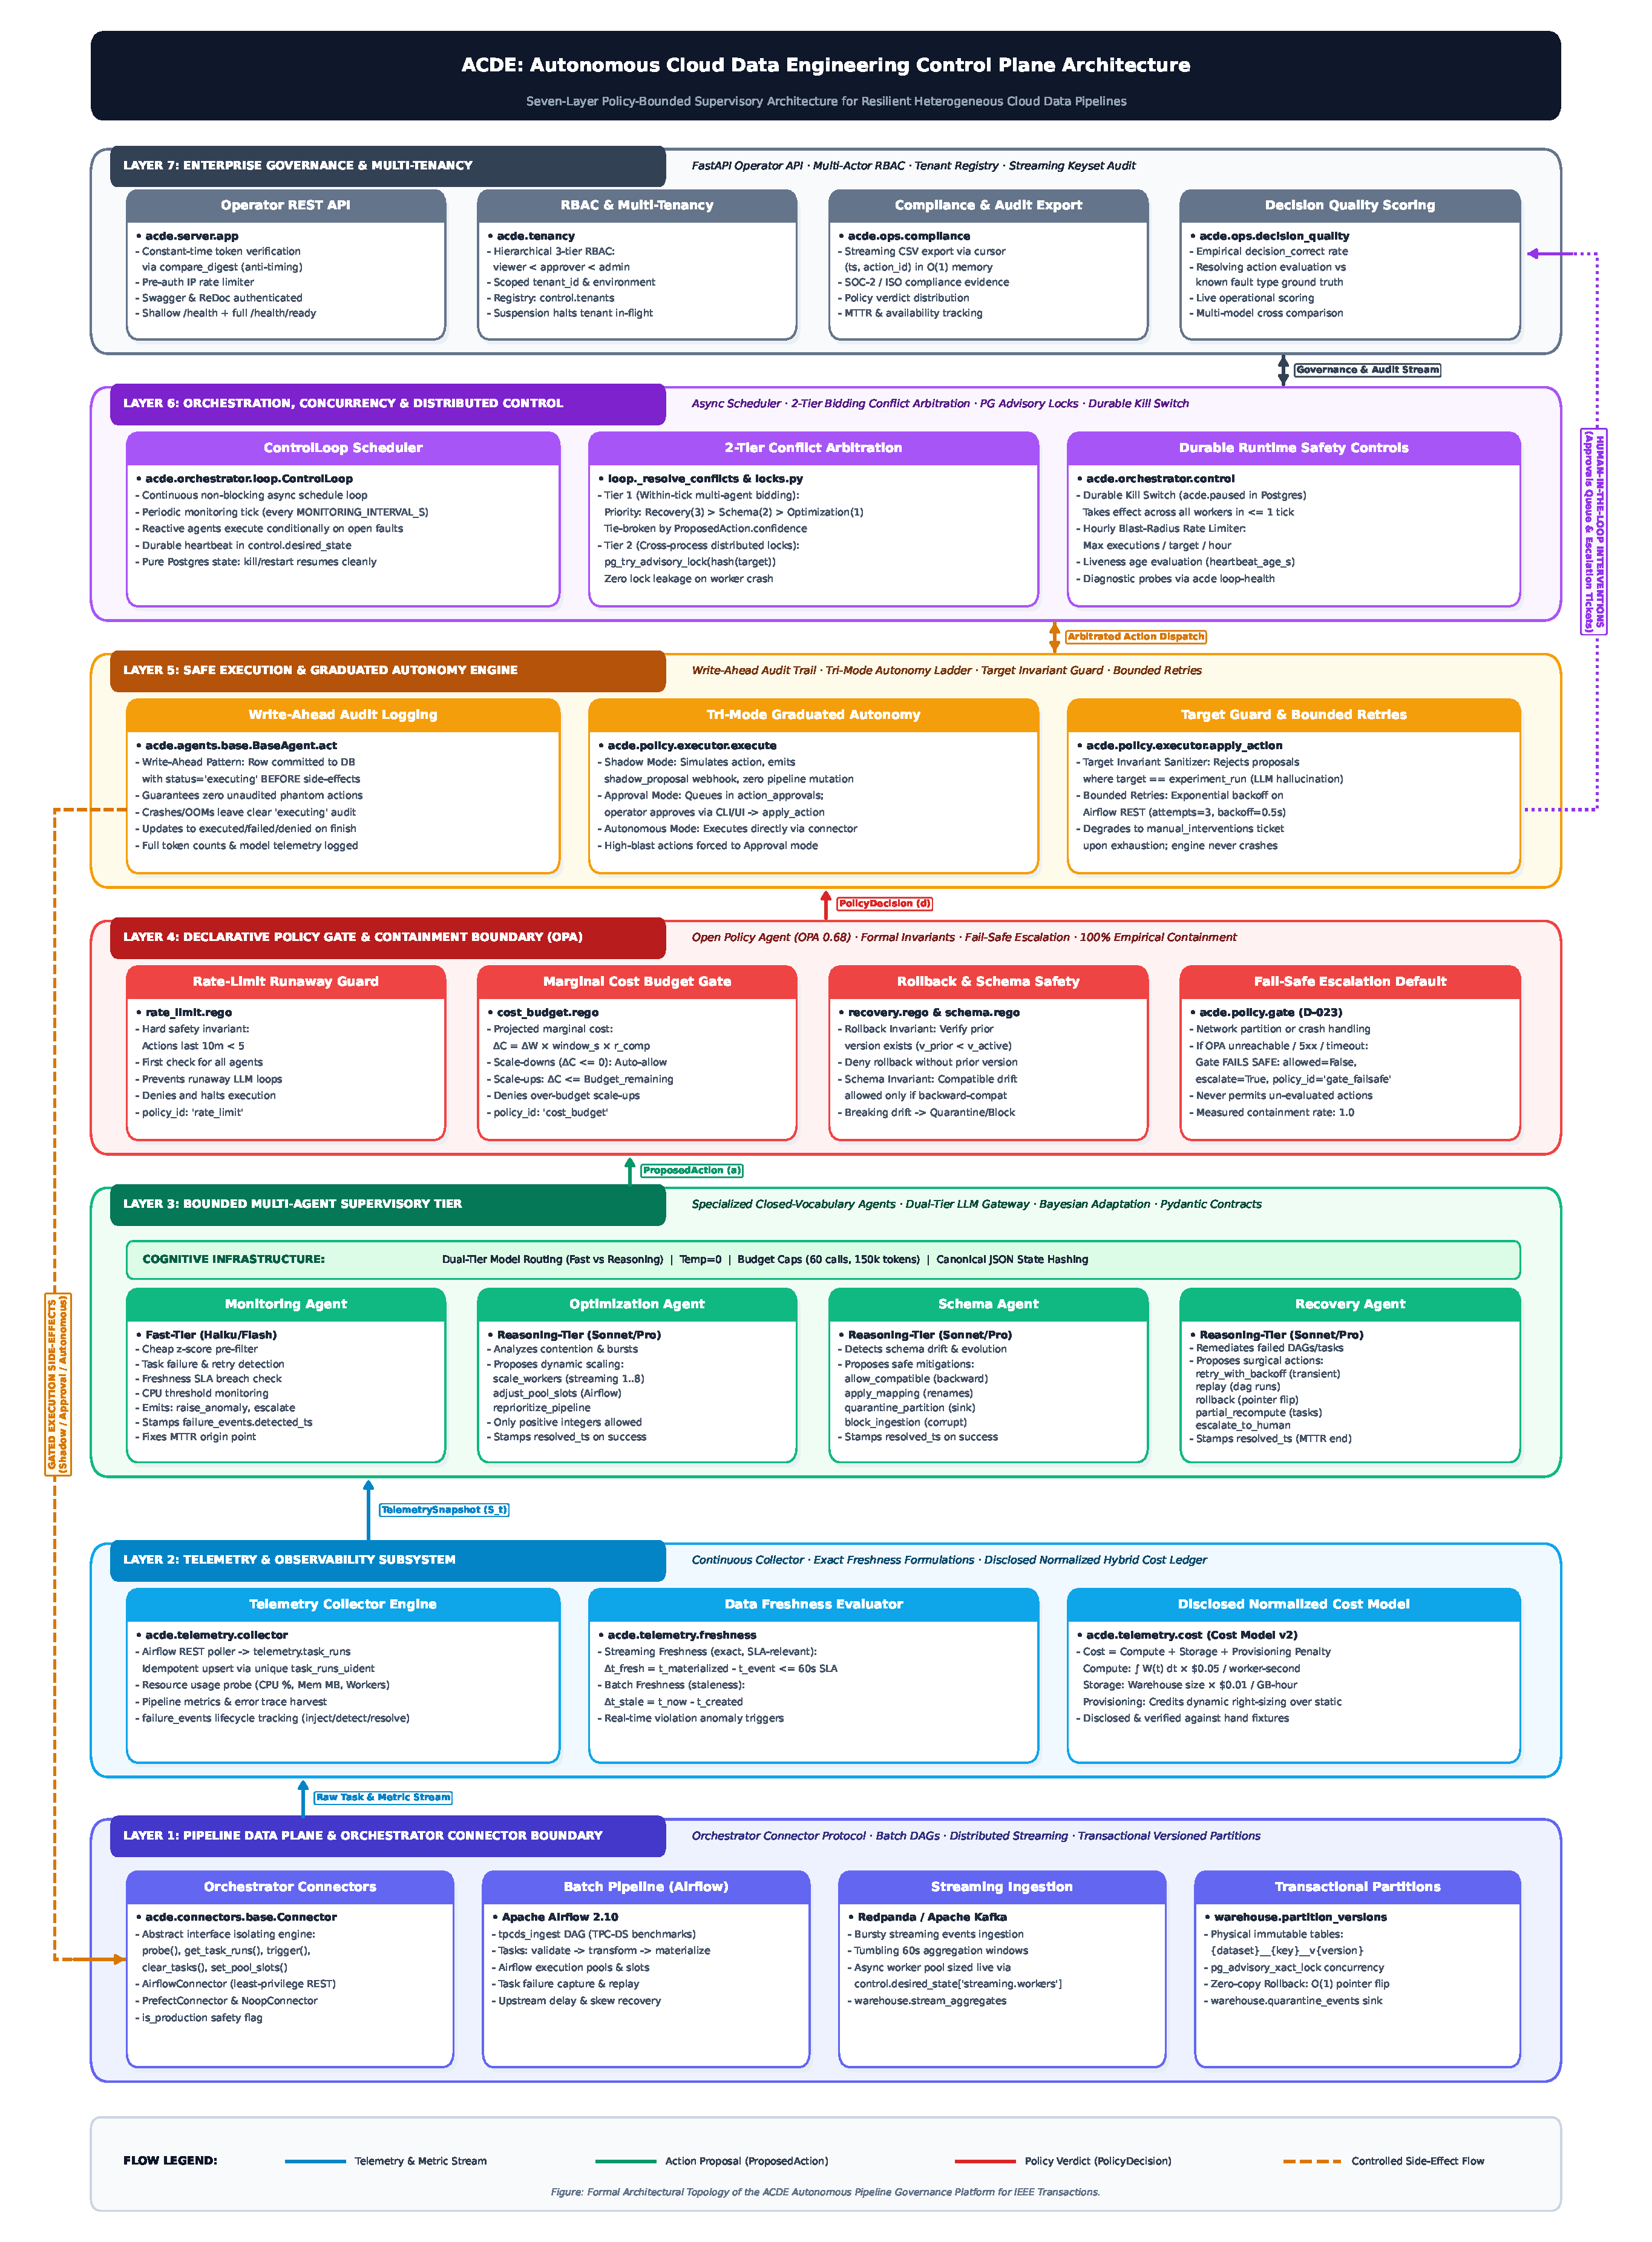
\includegraphics[width=0.98\textwidth]{system_architecture.pdf}
% \caption{The seven-layer system architecture of \textsc{Acde}, illustrating the data-flow progression from data plane execution up through autonomous multi-agent reasoning, declarative OPA policy gating, write-ahead safe execution, and multi-tenant enterprise governance.}
% \label{fig:system_architecture}
% \end{figure*}
%
% ------------------------------------------------------------------------------
% OPTION B: PURE TIKZ VECTOR FIGURE (COMPILED INLINE WITHOUT EXTERNAL ASSETS)
% ------------------------------------------------------------------------------
\begin{figure*}[!t]
\centering
\begin{tikzpicture}[
    >=stealth,
    node distance=1.2cm and 1.5cm,
    every text node part/.style={align=center},
    layer/.style={draw=black!75, rounded corners=3pt, line width=0.8pt, fill=blue!3, inner sep=6pt, text width=0.94\textwidth},
    subbox/.style={draw=black!60, rounded corners=2pt, line width=0.6pt, fill=white, inner sep=4pt},
    agentbox/.style={draw=teal!80, fill=teal!6, rounded corners=2pt, line width=0.6pt, inner sep=3pt},
    policybox/.style={draw=red!80, fill=red!5, rounded corners=2pt, line width=0.6pt, inner sep=3pt},
    databox/.style={draw=indigo!80, fill=indigo!5, rounded corners=2pt, line width=0.6pt, inner sep=3pt}
]

% Layer 7: Governance & Multi-Tenancy
\node[layer] (L7) {
    \textbf{\footnotesize Layer 7: Enterprise Governance \& Multi-Tenancy Plane (\texttt{acde.server}, \texttt{acde.tenancy})} \\
    \vspace{1pt}
    \begin{minipage}{0.92\textwidth}
    \centering
    \begin{tabular}{cccc}
        \fcolorbox{black!40}{white}{\scriptsize FastAPI Operator API (\texttt{compare\_digest} Auth)} &
        \fcolorbox{black!40}{white}{\scriptsize RBAC Engine ($\text{viewer} < \text{approver} < \text{admin}$)} &
        \fcolorbox{black!40}{white}{\scriptsize Tenant Registry (\texttt{control.tenants})} &
        \fcolorbox{black!40}{white}{\scriptsize Keyset Streaming Audit Export ($O(1)$ RAM)}
    \end{tabular}
    \end{minipage}
};

% Layer 6: Orchestration & Concurrency
\node[layer, below=0.35cm of L7] (L6) {
    \textbf{\footnotesize Layer 6: Orchestration, Concurrency \& Distributed Control Loop (\texttt{acde.orchestrator})} \\
    \vspace{1pt}
    \begin{minipage}{0.92\textwidth}
    \centering
    \begin{tabular}{cccc}
        \fcolorbox{black!40}{white}{\scriptsize Asynchronous Loop (\texttt{loop.ControlLoop})} &
        \fcolorbox{black!40}{white}{\scriptsize 2-Tier Bidding Conflict Arbitration} &
        \fcolorbox{black!40}{white}{\scriptsize PG Advisory Locks (\texttt{pg\_try\_advisory\_lock})} &
        \fcolorbox{black!40}{white}{\scriptsize Durable Kill Switch \& Liveness Heartbeat}
    \end{tabular}
    \end{minipage}
};

% Layer 5: Execution & Graduated Autonomy
\node[layer, below=0.35cm of L6] (L5) {
    \textbf{\footnotesize Layer 5: Safe Execution \& Graduated Autonomy Engine (\texttt{acde.policy.executor}, \texttt{acde.human.approvals})} \\
    \vspace{1pt}
    \begin{minipage}{0.92\textwidth}
    \centering
    \begin{tabular}{cccc}
        \fcolorbox{black!40}{white}{\scriptsize Write-Ahead Audit Trail (\texttt{status='executing'})} &
        \fcolorbox{black!40}{white}{\scriptsize Tri-Mode: $\text{Shadow} \rightarrow \text{Approval} \rightarrow \text{Autonomous}$} &
        \fcolorbox{black!40}{white}{\scriptsize Action Dispatcher \& Handlers (\texttt{apply\_action})} &
        \fcolorbox{black!40}{white}{\scriptsize Bounded Exponential Retries $\rightarrow$ Human Escalation}
    \end{tabular}
    \end{minipage}
};

% Layer 4: Policy Gate & OPA
\node[layer, below=0.35cm of L5, fill=red!2] (L4) {
    \textbf{\footnotesize Layer 4: Declarative Policy Gate \& Containment Boundary (\texttt{acde.policy.gate}, Open Policy Agent)} \\
    \vspace{1pt}
    \begin{minipage}{0.92\textwidth}
    \centering
    \begin{tabular}{cccc}
        \fcolorbox{red!70}{white}{\scriptsize Runaway Rate Guard ($\le 5\text{ ops}/10\text{min}$)} &
        \fcolorbox{red!70}{white}{\scriptsize Marginal Cost Budget Checker ($\Delta C \le B$)} &
        \fcolorbox{red!70}{white}{\scriptsize Versioned Rollback Invariant} &
        \fcolorbox{red!70}{white}{\scriptsize Fail-Safe Escalation Default}
    \end{tabular}
    \end{minipage}
};

% Layer 3: Bounded Multi-Agent Tier
\node[layer, below=0.35cm of L4, fill=teal!2] (L3) {
    \textbf{\footnotesize Layer 3: Bounded Multi-Agent Supervisory Tier (\texttt{acde.agents}, \texttt{acde.llm.client})} \\
    \vspace{1pt}
    \begin{minipage}{0.92\textwidth}
    \centering
    \begin{tabular}{cccc}
        \fcolorbox{teal!80}{white}{\scriptsize \textbf{Monitoring Agent} ($M_{\text{fast}}$, $z$-score filter)} &
        \fcolorbox{teal!80}{white}{\scriptsize \textbf{Optimization Agent} ($M_{\text{reasoning}}$, autoscale)} &
        \fcolorbox{teal!80}{white}{\scriptsize \textbf{Schema Agent} ($M_{\text{reasoning}}$, quarantine)} &
        \fcolorbox{teal!80}{white}{\scriptsize \textbf{Recovery Agent} ($M_{\text{reasoning}}$, rollback)}
    \end{tabular} \\
    \vspace{2pt}
    \begin{tabular}{ccc}
        \fcolorbox{teal!80}{white}{\scriptsize Closed Action Space Contract ($\mathcal{A}$ via Pydantic)} &
        \fcolorbox{teal!80}{white}{\scriptsize Dual-Tier LLM Gateway ($T=0$, Token Capping)} &
        \fcolorbox{teal!80}{white}{\scriptsize Clamped Bayesian Outcome Adaptation}
    \end{tabular}
    \end{minipage}
};

% Layer 2: Telemetry & Observability
\node[layer, below=0.35cm of L3] (L2) {
    \textbf{\footnotesize Layer 2: Telemetry \& Quantitative Cost Engine (\texttt{acde.telemetry})} \\
    \vspace{1pt}
    \begin{minipage}{0.92\textwidth}
    \centering
    \begin{tabular}{ccc}
        \fcolorbox{black!40}{white}{\scriptsize Continuous Freshness Evaluation ($\Delta t_{\text{fresh}} \le \text{SLA}$)} &
        \fcolorbox{black!40}{white}{\scriptsize Normalized Step-Integrated Cost Ledger} &
        \fcolorbox{black!40}{white}{\scriptsize Orchestrator Task \& Metric Harvest}
    \end{tabular}
    \end{minipage}
};

% Layer 1: Data Plane & Connectors
\node[layer, below=0.35cm of L2, fill=blue!2] (L1) {
    \textbf{\footnotesize Layer 1: Data Plane \& Orchestrator Connector Boundary (\texttt{acde.connectors}, \texttt{acde.dataplane})} \\
    \vspace{1pt}
    \begin{minipage}{0.92\textwidth}
    \centering
    \begin{tabular}{cccc}
        \fcolorbox{blue!80}{white}{\scriptsize Connector Protocol ($\mathcal{C}$): Airflow, Prefect, Noop} &
        \fcolorbox{blue!80}{white}{\scriptsize Immutable Versioned Partitions ($O(1)$ Pointer Flip)} &
        \fcolorbox{blue!80}{white}{\scriptsize Tumbling Window Streaming Aggregates} &
        \fcolorbox{blue!80}{white}{\scriptsize Quarantine Sink Table}
    \end{tabular}
    \end{minipage}
};

% Arrows
\draw[->, line width=1pt] (L1) -- node[right, font=\tiny] {Raw Telemetry} (L2);
\draw[->, line width=1pt] (L2) -- node[right, font=\tiny] {State Snapshot $\mathcal{S}_t$} (L3);
\draw[->, line width=1pt] (L3) -- node[right, font=\tiny] {ProposedAction $\mathbf{a}$} (L4);
\draw[->, line width=1pt] (L4) -- node[right, font=\tiny] {PolicyDecision $\mathbf{d}$} (L5);
\draw[<->, line width=1pt] (L5) -- node[right, font=\tiny] {Arbitrated Action Execution} (L6);
\draw[<->, line width=1pt] (L6) -- node[right, font=\tiny] {Control \& Governance State} (L7);

% Feedback Side-channel
\draw[->, dashed, line width=0.8pt, black!60] (L5.west) to[out=180,in=180] node[left, font=\tiny] {Controlled Side-Effects} (L1.west);

\end{tikzpicture}
\caption{The seven-layer system architecture of \textsc{Acde}, illustrating the data-flow progression from data plane execution up through autonomous multi-agent reasoning, declarative OPA policy gating, write-ahead safe execution, and multi-tenant enterprise governance.}
\label{fig:system_architecture}
\end{figure*}

\subsection{Formal Contract and State Space Foundations}
\label{subsec:contracts}

The entire operational state of \textsc{Acde} is captured as a deterministic telemetry snapshot $\mathcal{S}_t \in \mathbf{S}$ evaluated at discrete control cycles $t$:
\begin{equation}
\mathcal{S}_t = \big\langle \mathbf{T}_t, \mathbf{R}_t, \mathbf{M}_t, \sigma_t, \mathbf{F}_t^{\text{open}} \big\rangle
\end{equation}
where $\mathbf{T}_t$ represents normalized task execution observations ($\text{state} \in \{\text{success}, \text{failed}, \text{retry}\}$), $\mathbf{R}_t$ denotes point-in-time compute utilization vectors $(\text{cpu\_pct}, \text{mem\_mb}, \text{workers})$, $\mathbf{M}_t$ maps pipeline identifiers to quantitative health metrics, $\sigma_t \in \{\text{backward}, \text{breaking}, \text{unknown}\}$ defines schema compatibility status, and $\mathbf{F}_t^{\text{open}}$ is the set of unmitigated fault records.

To guarantee that autonomous agents can never act as vector injection surfaces, all agent outputs are strictly restricted to a closed contract schema:
\begin{equation}
\mathbf{a} = \big\langle \text{id}, \text{agent}, \text{type}, \text{target}, \mathbf{p}, \text{justification}, c \big\rangle \in \mathcal{A}
\end{equation}
where $\text{agent} \in \{\text{monitoring}, \text{optimization}, \text{schema}, \text{recovery}\}$, $\text{type} \in \mathbf{\Omega}_{\text{agent}}$ is bounded to a predefined discrete action vocabulary, $\text{target}$ identifies the pipeline or dataset entity, $\mathbf{p} \in \mathbb{R}^k$ represents validated numeric control parameters (e.g., worker count $n_{\text{workers}} \in \mathbb{Z}^+$), and $c \in [0, 1]$ denotes the agent's proposal confidence.

\subsection{Data Plane and Orchestrator Connector Abstraction}
\label{subsec:dataplane}

The Data Plane hosts production workloads across dual modalities:
\begin{enumerate}
    \item \textbf{Batch Processing Substrate}: Managed via orchestrators (e.g., Apache Airflow, Prefect). Workloads ingest and materialize versioned datasets into relational storage.
    \item \textbf{Streaming Processing Substrate}: Powered by distributed message brokers (e.g., Apache Kafka, Redpanda). Workers continuously process incoming records into discrete tumbling windows ($W_{\text{size}} = 60\,\text{s}$). The pool of active streaming workers $W_{\text{stream}} \in [1, 8]$ is dynamically sized via control-plane state.
\end{enumerate}

\subsubsection{Connector Boundary}
To isolate the governance engine from orchestrator-specific APIs, \textsc{Acde} defines an extensible connector interface $\mathcal{C}$:
\begin{equation}
\mathcal{C} = \big\langle \text{health}(), \text{get\_task\_runs}(), \text{trigger}(), \text{clear\_tasks}(), \text{set\_pool}() \big\rangle
\end{equation}
Concrete implementations include the \texttt{AirflowConnector} (interfacing via authenticated REST endpoints with bounded retry backoff), \texttt{PrefectConnector}, and \texttt{NoopConnector} (for non-intrusive observation).

\subsubsection{Transactional Partition Versioning and Zero-Copy Rollback}
Data state integrity is maintained through an append-only versioning substrate in the warehouse schema. For any dataset $d$ and partition key $p$, physical tables follow the deterministic naming schema:
\begin{equation}
\text{table\_name}(d, p, v) = \text{slug}(d) \parallel \text{"\_\_"} \parallel \text{slug}(p) \parallel \text{"\_\_v"} \parallel v
\end{equation}
Active dataset views resolve to the specific physical version marked $\text{active} = \text{True}$ in the catalog $\texttt{warehouse.partition\_versions}$. To eliminate race conditions during concurrent DAG materializations, version allocation executes within an ACID transaction guarded by a 32-bit PostgreSQL advisory transaction lock:
\begin{equation}
\mathcal{K}_{\text{lock}}(d, p) = \Big(\text{int}\big(\text{SHA256}(d \parallel \text{":"} \parallel p)[0:4]\big) - 2^{31}\Big) \in \mathbb{Z}_{\text{signed32}}
\end{equation}
Rollback from version $v$ to predecessor $v-1$ is achieved in $O(1)$ time via a single transactional metadata pointer flip:
\begin{equation}
\begin{aligned}
\text{UPDATE } & \texttt{warehouse.partition\_versions} \\
\text{SET } & \text{active} = (\text{version} = v - 1) \\
\text{WHERE } & \text{dataset} = d \land \text{partition\_key} = p
\end{aligned}
\end{equation}
Physical data is never duplicated or destroyed during rollback, ensuring instant recovery without I/O overhead.

\subsection{Telemetry Engine and Disclosed Normalized Cost Model}
\label{subsec:telemetry}

\subsubsection{Data Freshness Formulations}
Freshness is continuously tracked across both streaming and batch modalities:
\begin{align}
\Delta t_{\text{freshness}}^{\text{stream}} &= t_{\text{materialized}} - \max(t_{\text{event}}) \label{eq:stream_fresh} \\
\Delta t_{\text{staleness}}^{\text{batch}} &= t_{\text{now}} - t_{\text{created}} \label{eq:batch_fresh}
\end{align}
An SLA violation occurs whenever $\Delta t_{\text{freshness}}^{\text{stream}} > \tau_{\text{SLA}}$ (where $\tau_{\text{SLA}} = 60\,\text{s}$).

\subsubsection{Disclosed Hybrid Cost Model}
Unlike proprietary cloud governance platforms that obscure cost formulations, \textsc{Acde} discloses a two-tier cost model that quantifies active compute, persisted storage, and avoided over-provisioning:
\begin{equation}
C_{\text{total}} = C_{\text{compute}} + C_{\text{storage}} + C_{\text{provisioning}}
\label{eq:cost_total}
\end{equation}
Active compute cost integrates resource units over time windows $[t_0, t_1]$:
\begin{equation}
C_{\text{compute}} = r_{\text{comp}} \sum_{k \in \{\text{stream}, \text{batch}\}} \int_{t_0}^{t_1} W_k(t) \, dt
\end{equation}
where $W_k(t)$ is the step-integrated worker count and $r_{\text{comp}} = \$0.05 / (\text{unit}\cdot\text{s})$. Persisted storage is computed from catalog relation byte sizes:
\begin{equation}
C_{\text{storage}} = r_{\text{stor}} \cdot S_{\text{warehouse}}^{\text{GB}}(t_1)
\end{equation}
where $r_{\text{stor}} = \$0.01 / (\text{GB}\cdot\text{hour})$. Finally, avoided over-provisioning credits dynamic right-sizing:
\begin{equation}
C_{\text{provisioning}} = r_{\text{comp}} \cdot U_{\text{alloc}}(\text{config}) \cdot T_{\text{horizon}}
\end{equation}
Static baseline configurations hold fixed allocations ($U_{\text{alloc}} = 4\,\text{units}$), whereas dynamic configurations holding right-sizing agents require only $U_{\text{alloc}} = 2\,\text{units}$ over horizon $T_{\text{horizon}} = 3600\,\text{s}$.

\subsection{Bounded Multi-Agent Supervisory Tier}
\label{subsec:agents}

\textsc{Acde} structures operational autonomy through four bounded, specialized supervisory agents. Table~\ref{tab:agent_spec} details their respective action alphabets, preconditions, gating invariants, and operational effects.

\begin{table*}[!t]
\centering
\caption{Formal Specification of \textsc{Acde} Supervisory Agents, Discrete Action Spaces, and Operational Invariants}
\label{tab:agent_spec}
\footnotesize
\begin{tabularx}{\textwidth}{l p{2.8cm} p{2.8cm} p{3.2cm} X}
\toprule
\textbf{Agent} & \textbf{Action Type ($\mathbf{\Omega}$)} & \textbf{Target Entity} & \textbf{Preconditions / Triggers} & \textbf{Operational Effect \& Resolution} \\
\midrule
\multirow{3}{*}{\textbf{Monitoring}} 
& \texttt{raise\_anomaly} & Pipeline / Component & $z(\mathbf{x}) \ge \theta_z \lor \text{task\_state}=\text{fail}$ & Records incident; stamps \texttt{detected\_ts} (MTTR origin). \\
& \texttt{escalate} & Service / Incident & Multi-point anomaly saturation & Creates urgent human intervention record. \\
& \texttt{no\_action} & None & Pipeline within normal thresholds & No side-effect; heartbeats telemetry loop. \\
\midrule
\multirow{4}{*}{\textbf{Optimization}} 
& \texttt{scale\_workers} & Streaming Service & Ingress surge; $\Delta t_{\text{fresh}} > \tau_{\text{SLA}}$ & Resizes worker pool ($n \in [1, 8]$); stamps \texttt{resolved\_ts}. \\
& \texttt{adjust\_pool\_slots} & Airflow Pool & Task queue backlog; contention & Updates orchestrator execution slots; stamps \texttt{resolved\_ts}. \\
& \texttt{reprioritize\_pipeline} & Pipeline ID & Criticality SLA breach & Reprioritizes DAG scheduling order. \\
& \texttt{no\_action} & None & Sufficient resource headroom & No resource modification. \\
\midrule
\multirow{5}{*}{\textbf{Schema}} 
& \texttt{allow\_compatible} & Dataset Partition & $\sigma_t = \text{backward}$ drift & Acknowledges non-breaking column evolution. \\
& \texttt{apply\_mapping} & Dataset ID & Alias / Renaming drift & Updates runtime projection mapping in control catalog. \\
& \texttt{quarantine\_partition} & Dataset Partition & $\sigma_t = \text{breaking}$ drift & Sets $\text{active}=\text{False}$; routes payload to quarantine sink table. \\
& \texttt{block\_ingestion} & Dataset / Upstream & Persistent corrupt stream & Sets $\texttt{ingestion.blocked}=1$; halts ingestion pipeline. \\
& \texttt{no\_action} & None & Schema matches registered contract & Preserves active ingestion. \\
\midrule
\multirow{6}{*}{\textbf{Recovery}} 
& \texttt{retry\_with\_backoff} & DAG / Task Run & Transient orchestrator / network fault & Dispatches delayed replay through orchestrator API. \\
& \texttt{replay} & DAG Run ID & Mid-pipeline execution failure & Triggers full pipeline replay with original parameters. \\
& \texttt{rollback} & Dataset Partition & Corrupted data materialization & Transactional pointer flip to prior version ($v - 1$). \\
& \texttt{partial\_recompute} & Failed Task Subgraph & Upstream failure in DAG graph & Clears failed task states; retains succeeded upstream nodes. \\
& \texttt{escalate\_to\_human} & Unrecoverable State & Missing prior version; persistent crash & Dispatches alert; enqueues manual intervention ticket. \\
& \texttt{no\_action} & None & No open failure events & Dormant monitor mode. \\
\bottomrule
\end{tabularx}
\end{table*}

\subsubsection{Dual-Tier LLM Architecture and Token Guarding}
To minimize operational cost while maintaining high reasoning quality, agents leverage a two-tier model hierarchy:
\begin{itemize}
    \item \textbf{Fast-Tier Models ($M_{\text{fast}}$)}: Low-latency, cost-effective models (e.g., Claude 3.5 Haiku, Gemini 2.5 Flash) handle continuous, high-frequency anomaly monitoring.
    \item \textbf{Reasoning-Tier Models ($M_{\text{reasoning}}$)}: High-capacity models (e.g., Claude 3.7 Sonnet, Gemini 2.5 Pro) are invoked strictly upon detection of open failure incidents.
\end{itemize}
All inferences enforce strict deterministic settings (temperature $T = 0$). To prevent runaway cost during cascading failures, each governance run is bound by hard call and token caps:
\begin{equation}
N_{\text{calls}} \le K_{\max} \quad (60), \quad N_{\text{tokens}} \le T_{\max} \quad (150{,}000)
\end{equation}
Furthermore, the agent client hashes identical telemetry snapshots $\text{SHA256}(\mathcal{S}_t^{\text{canon}})$ to cache proposals across repeated cycles.

\subsubsection{Statistical Anomaly Pre-Filtering}
Before invoking any model, the Monitoring Agent executes a lightweight, deterministic statistical pre-filter:
\begin{equation}
z(x_t) = \frac{x_t - \mu_w}{\sigma_w}
\end{equation}
evaluated over a rolling observation window $w$. Anomalies are flagged if $|z(x_t)| > \theta_z$, if task run states enter $\{\text{failed}, \text{up\_for\_retry}\}$, or if CPU utilization exceeds $\theta_{\text{cpu}} = 80\%$. Newly detected anomalies are immediately written to $\texttt{telemetry.failure\_events}$, providing same-tick visibility to reactive agents and fixing the baseline timestamp for Mean Time to Resolution ($\text{MTTR} = t_{\text{resolved}} - t_{\text{detected}}$).

\subsubsection{Bounded Empirical Adaptation Engine}
Rather than allowing unconstrained prompt mutation, \textsc{Acde} supports bounded adaptation by computing empirical action success priors over historical runs:
\begin{equation}
P(\text{success} \mid a, f) = \frac{\sum \mathbf{1}(\text{resolved} \land \text{action}=a \land \text{fault}=f)}{\sum \mathbf{1}(\text{executed} \land \text{action}=a \land \text{fault}=f)}
\label{eq:prior}
\end{equation}
If no prior exists, a neutral prior $P_0 = 0.5$ is assumed. The effective proposal confidence is updated via bounded Bayesian blending:
\begin{equation}
c_{\text{adapted}} = \max\Big(c_{\min}, \min\big(c_{\max}, (1 - w_{\text{adapt}}) c_{\text{base}} + w_{\text{adapt}} P(\text{success} \mid a, f)\big)\Big)
\label{eq:blend}
\end{equation}
where $w_{\text{adapt}} = 0.3$, $c_{\min} = 0.1$, and $c_{\max} = 0.95$. This guarantees that empirical history dynamically prioritizes effective remediations without ever bypassing declarative policy gates.

\subsection{Declarative Policy Gate and Containment Boundary}
\label{subsec:policy}

The central safety guarantee of \textsc{Acde} is that \emph{no proposed action touches physical infrastructure without formal policy certification}. The Open Policy Agent (OPA) evaluates each proposal $\mathbf{a}$ against declarative Rego policies over assembled context $\mathcal{K}_t$:
\begin{equation}
\mathcal{D} = \text{OPA}\big(\text{input} = \langle \mathbf{a}, \mathcal{K}_t \rangle\big) \rightarrow \langle \text{allowed}, \text{escalate}, \text{reason}, \text{policy\_id} \rangle
\end{equation}

\subsubsection{Formal Safety Invariants}
The policy gate enforces four foundational invariants:
\begin{enumerate}
    \item \textbf{Rate-Limit Runaway Guard}: Prevents agent loop cascades by rejecting actions if an agent has executed $\ge 5$ actions within a 10-minute sliding window:
    \begin{equation}
    \mathcal{I}_{\text{rate}} \iff \big|\{ \mathbf{a}' \in \mathcal{H}_{\text{actions}} \mid t - t_{\mathbf{a}'} \le 600\,\text{s} \land \mathbf{a}'.\text{agent} = \mathbf{a}.\text{agent} \}\big| < 5
    \end{equation}
    \item \textbf{Marginal Cost Budget Bound}: Restricts worker scale-ups such that projected marginal cost does not exceed remaining budget $B_t$:
    \begin{equation}
    \Delta C_{\text{marginal}} = (n_{\text{target}} - n_{\text{current}}) \cdot \Delta t_{\text{window}} \cdot r_{\text{comp}} \le B_t
    \end{equation}
    Scale-down actions ($\Delta C_{\text{marginal}} \le 0$) are always unconditionally approved.
    \item \textbf{Versioned Rollback Safety Invariant}: Rollback actions are certified if and only if a valid prior version exists:
    \begin{equation}
    \mathcal{I}_{\text{rollback}} \iff \exists v_{\text{prior}} \in \texttt{warehouse.partition\_versions} \text{ s.t. } v_{\text{prior}} < v_{\text{active}}
    \end{equation}
    Rollbacks targeting non-existent predecessors are blocked and escalated.
    \item \textbf{Schema Compatibility Invariant}: Actions declaring schema compatibility are denied if drift is breaking:
    \begin{equation}
    \mathcal{I}_{\text{schema}} \iff (\mathbf{a}.\text{type} \in \mathbf{\Omega}_{\text{compat}} \land \sigma_t = \text{backward}) \lor (\mathbf{a}.\text{type} \in \mathbf{\Omega}_{\text{contain}})
    \end{equation}
\end{enumerate}

\subsubsection{Fail-Safe Fallback Principle}
If the policy engine becomes unreachable due to network partitions or process crashes, the gate fails safe:
\begin{equation}
\text{status}(\text{OPA}) \neq 200 \implies \mathcal{D} = \langle \text{allowed} = \text{False}, \text{escalate} = \text{True}, \text{"gate\_failsafe"} \rangle
\end{equation}
Under no circumstance does an outage degrade into unconstrained autonomous execution.

\subsection{Concurrency Control, Bidding Arbitration, and Safe Execution}
\label{subsec:execution}

\subsubsection{Two-Tier Conflict Arbitration}
When multiple reactive agents observe an incident simultaneously, they may propose conflicting actions targeting the same entity. \textsc{Acde} resolves this through a two-tier arbitration mechanism:
\begin{enumerate}
    \item \textbf{Tier 1: Multi-Agent Priority Bidding}: Contending proposals within a single loop tick are ranked lexicographically by agent criticality tier and proposal confidence:
    \begin{equation}
    \text{Rank}(\mathbf{a}) = \big\langle \text{Tier}(\mathbf{a}.\text{agent}), \, \mathbf{a}.\text{confidence} \big\rangle
    \end{equation}
    where $\text{Tier}(\text{recovery}) = 3 > \text{Tier}(\text{schema}) = 2 > \text{Tier}(\text{optimization}) = 1$. The highest-ranking proposal wins the target; losing proposals are logged as outbid.
    \item \textbf{Tier 2: Cross-Process Advisory Locking}: To prevent race conditions across horizontally distributed \textsc{Acde} instances, winning actions must acquire a non-blocking PostgreSQL session advisory lock on the target entity:
    \begin{equation}
    \text{acquired} \leftarrow \texttt{pg\_try\_advisory\_lock}\big(\text{int32}(\text{SHA256}(\mathbf{a}.\text{target}))\big)
    \end{equation}
    If unacquired, execution skips cleanly without blocking worker threads.
\end{enumerate}

\subsubsection{Write-Ahead Audit Trail and Target Sanitization}
Prior to invoking external side-effects, the executor writes an intent record into $\texttt{telemetry.agent\_actions}$ with $\text{status} = \texttt{"executing"}$. In the event of an infrastructure crash or host reboot mid-execution, the audit log unambiguously identifies in-flight operations. Furthermore, to guard against live LLM hallucinations (such as models echoing run identifiers as action targets), an invariant sanitizer rejects invalid targets before calling orchestrator APIs.

\subsubsection{Graduated Autonomy Ladder}
Allowed actions execute under one of three graduated autonomy modes:
\begin{itemize}
    \item \textbf{Shadow Mode}: Logs intended operations and dispatches webhooks without mutating pipeline state.
    \item \textbf{Approval Mode}: Enqueues actions into $\texttt{telemetry.action\_approvals}$ for operator sign-off via CLI or dashboard.
    \item \textbf{Autonomous Mode}: Executes side effects directly via connectors with bounded exponential retry backoff (3 attempts, max backoff 5\,s). High-blast-radius actions can be selectively held in Approval mode.
\end{itemize}

Algorithm~\ref{alg:control_loop} formally outlines the end-to-end execution of the \textsc{Acde} control loop.

% ------------------------------------------------------------------------------
% ALGORITHM 1: ACDE CONTROL LOOP
% ------------------------------------------------------------------------------
\begin{algorithm}[!t]
\caption{\textsc{Acde} Autonomous Supervisory Control Loop}
\label{alg:control_loop}
\begin{algorithmic}[1]
\Require Interval $\Delta t$, Configuration $\mathbf{C}$, Remaining Budget $B$
\State Initialize connector $\mathcal{C}$, OPA client, PostgreSQL connection pool
\While{$\text{stop\_signal} = \text{False}$}
    \State $\texttt{record\_heartbeat}()$; \Comment{Stamp liveness in catalog}
    \If{$\texttt{is\_paused}() \lor \texttt{kill\_switch\_engaged}()$}
        \State $\texttt{sleep}(\Delta t)$; \textbf{continue}
    \EndIf
    \State $\mathcal{S}_t \leftarrow \texttt{observe\_telemetry}()$
    \If{$\text{monitoring} \in \mathbf{C}.\text{enabled}$}
        \State $\mathbf{a}_{\text{mon}} \leftarrow \texttt{MonitoringAgent}.\text{reason}(\mathcal{S}_t)$
        \State $\texttt{execute\_action}(\mathbf{a}_{\text{mon}})$
    \EndIf
    \State $\mathbf{F}_{\text{open}} \leftarrow \texttt{query\_open\_faults}()$
    \If{$|\mathbf{F}_{\text{open}}| > 0$}
        \State $\mathbf{P} \leftarrow \emptyset$
        \For{$\text{agent} \in \{\text{schema}, \text{recovery}, \text{optimization}\}$}
            \If{$\text{agent} \in \mathbf{C}.\text{enabled}$}
                \State $\mathbf{a} \leftarrow \texttt{Agent}[\text{agent}].\text{reason}(\mathcal{S}_t)$
                \If{$\mathbf{a}.\text{type} \neq \texttt{"no\_action"}$}
                    \State $\mathbf{P} \leftarrow \mathbf{P} \cup \{\mathbf{a}\}$
                \EndIf
            \EndIf
        \EndFor
        \State $\mathbf{W}, \mathbf{L} \leftarrow \texttt{ArbitrateBids}(\mathbf{P})$ \Comment{Sort by Tier and Confidence}
        \For{$\mathbf{a}^* \in \mathbf{W}$}
            \If{$\texttt{blast\_radius\_exceeded}(\mathbf{a}^*.\text{target})$}
                \State \textbf{continue}
            \EndIf
            \With{$\texttt{target\_advisory\_lock}(\mathbf{a}^*.\text{target})$}
                \State $\mathcal{K}_t \leftarrow \texttt{build\_policy\_context}(\mathbf{a}^*, B)$
                \State $\mathcal{D} \leftarrow \texttt{evaluate\_opa}(\mathbf{a}^*, \mathcal{K}_t)$
                \State $\texttt{write\_ahead\_log}(\mathbf{a}^*, \mathcal{D}, \text{status}=\texttt{"executing"})$
                \If{$\mathcal{D}.\text{allowed}$}
                    \State $\text{res} \leftarrow \texttt{apply\_graduated\_execution}(\mathbf{a}^*, \mathcal{D})$
                \ElsIf{$\mathcal{D}.\text{escalate}$}
                    \State $\texttt{escalate\_to\_human}(\mathbf{a}^*, \mathcal{D}.\text{reason})$
                \EndIf
                \State $\texttt{update\_audit\_status}(\mathbf{a}^*.\text{id}, \text{res})$
            \EndWith
        \EndFor
    \EndIf
    \State $\texttt{sleep}(\Delta t)$
\EndWhile
\end{algorithmic}
\end{algorithm}

\subsection{Enterprise Multi-Tenancy, Security, and Governance Plane}
\label{subsec:enterprise}

The upper boundary of \textsc{Acde} provides enterprise-grade tenancy, authentication, and compliance auditing:
\begin{enumerate}
    \item \textbf{Cryptographic Constant-Time Authentication}: Requests to the operator API are authenticated via API keys or HTTP Basic credentials verified using constant-time digest comparison (\texttt{compare\_digest}), preventing timing-attack key recovery.
    \item \textbf{Role-Based Access Control (RBAC)}: Users are bound to hierarchical roles ($\text{viewer} < \text{approver} < \text{admin}$). Write operations, kill switches, and approval decisions require verified minimum privilege levels.
    \item \textbf{Multi-Tenant Isolation}: Telemetry, fault records, cost ledgers, and action audit rows are strictly scoped by $\texttt{tenant\_id}$ and $\texttt{environment}$. A centralized tenant registry ($\texttt{control.tenants}$) provides administrative activation and suspension lifecycle management.
    \item \textbf{Streaming Keyset Audit Pagination}: To facilitate external regulatory compliance (e.g., SOC-2, ISO 27001), audit queries implement keyset cursor pagination over $(\text{ts}, \text{action\_id})$. This enables continuous, memory-bounded ($O(1)$ RAM) streaming export of millions of historical governance decisions.
\end{enumerate}
